\section{Basic Hardware Construction in Chisel}
\label{sec:basic}
The Chisel constructs presented in the previous chapter are adequate
for most hardware circuits. We have in fact built an entire floating
point library using only those constructs. Occasionally, users might
want to leverage syntax for hardware facilities available in a
target backend from within Chisel. Suppose for example that a user is
having Chisel target a backend that has support for highly optimized
FFT circuits. One way to leverage this facility is to introduce a new
type of {\tt Node} into Chisel that maps directly to that syntax in
the backend. This approach keeps the Chisel graph sparse since all the
hardware construction complexity is pushed into the backends where the
backend synthesis tools could possibly map the hardware facility to
very dense circuits. The downside to this approach is that Chisel code
using {\tt Nodes} designed to target these backend hardware facilities
now have a strong dependence on that backend. Furthermore, targeting a
new backend would require effort to port the Chisel user code if the
new backend does not have built-in support for the hardware facility.

The nuts and bolts to pay attention to when implementing a new 
{\tt Node} are the node's code generation functions and the node's
inputs list. Let's say we are implementing a new {\tt Node} called
{\tt Foo}. If {\tt Foo}'s code generation function need to reference
nodes {\tt B}, {\tt A}, and {\tt R}, then all three of those nodes
must go into {\tt Foo}'s input list. Omitting a node can lead to a
scenario where Chisel is unable to reach the omitted node and thus
never emits the backend code for that node. The result is 
{\tt Foo}'s backend code will make reference to non-existing hardware.
This chapter will show how {\tt ListLookup} and {\tt Vec} nodes can be
implemented to target Verilog's case statements and arrays.

\subsection{ListLookup}
\begin{figure}[htb]
\centering
  \begin{subfigure}[t]{0.48\textwidth}
  \centering
  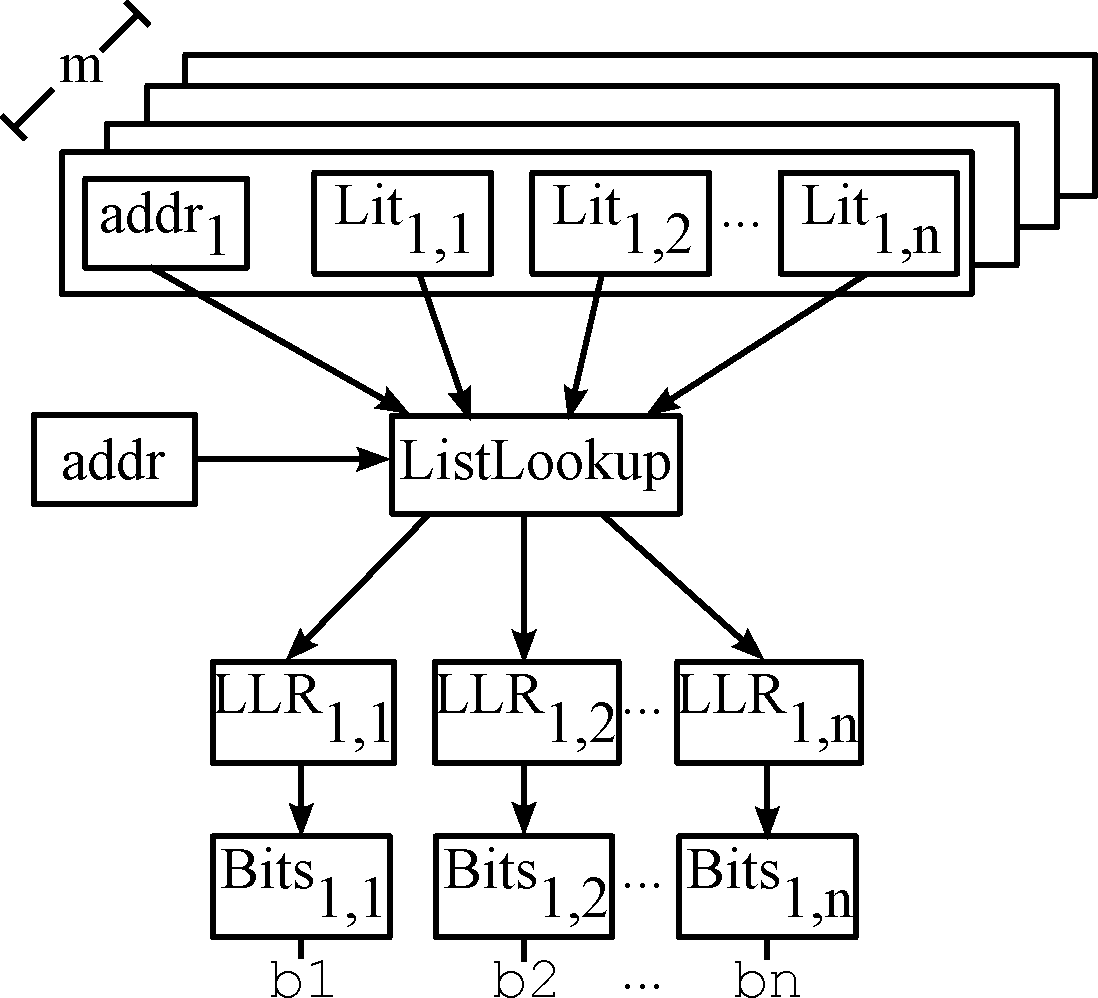
\includegraphics[width=\textwidth]{figures/listlookupnode.pdf}
  \caption{{\bf ListLookup Node}. Lit = {\tt Literal} node, LLR =
    {\tt ListLookupRef} nodes, and addr is shorthand for a {\tt Bits} node
    used as an address. Boxes with {\tt (addr$_j$,
      lits$_{i,j}$)} represent Scala tuples.}
  \label{fig:llnode}
  \end{subfigure}
  \hfill
  \begin{subfigure}[t]{0.48\textwidth}
  \centering
  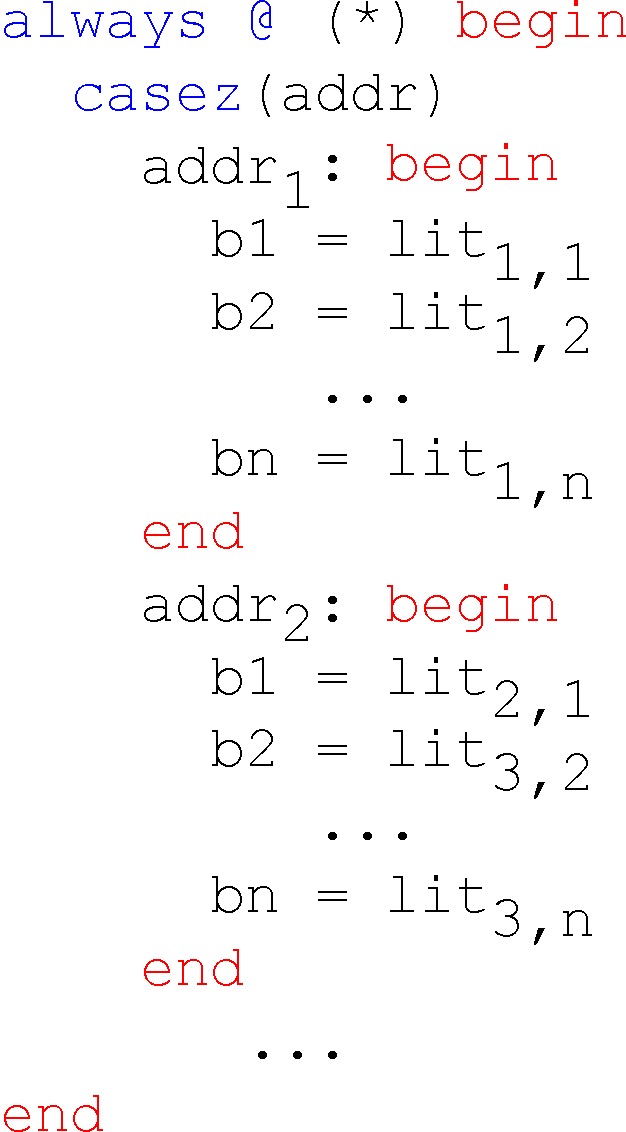
\includegraphics[width=0.5\textwidth]{figures/listlookupv.pdf}
  \caption{{\bf Generated ListLookup Code}. There are $m$ generated
    case statements each with $n$ literal assignments.}
  \label{fig:llv}
  \end{subfigure}
\caption{{\bf ListLookup}}
\label{fig:ll}
\end{figure}

\begin{verbbox}
ListLookup(addr: Bits, default: List[Lit], 
                       mapping: List[(addr, List[Lit])])
\end{verbbox}

We introduce {\tt ListLookup} and {\tt ListLookupRef} nodes to target
Verilog's case statement from within Chisel which is useful for
writing decode tables.

\textbf{ListLookup Node}.The inputs to this node, see
Figure~\ref{fig:llsyntax}, are an address, a default list of literals,
and a list of tuples {\tt (a$_i$, lits$_i$)} where {\tt lits$_i$} is a list
of a literals. Figure~\ref{fig:llnode} shows how the inputs to the
{\tt ListLookup} nodes are managed. This node is different from other
nodes in that it does not have an entry for {\tt emitDec} and {\tt
emitRef}. The only code generation function it fills out is the {\tt
emitDef} function which generates the case statements in
Figure~\ref{fig:llv}. The ListLookup generates a case statement for
every {\tt (a$_i$, lits$_i$)} tuple where each case statements will
have an assignment for each literal in {\tt lits$_i$}. The address
input to the ListLookup is used as the lookup address into the case
statement and the {\tt a$_i$}'s are used to match against the
address. If no address matches, the default assignment is used.

\begin{figure}
\centering
\theverbbox
\caption{ListLookup Syntax}
\label{fig:llsyntax}
\end{figure}

\textbf{ListLookupRef Node}. Creating a new {\tt ListLookup} will not return
the {\tt ListLookup} to the user, rather, a list of 
{\tt ListLookupRef} nodes are returned instead. The length of the 
{\tt ListLookupRef} list matches the length of {\tt lits$_i$}. 
{\tt ListLookupRef} nodes do not have an entry for {\tt emitDef} since
the assignments to these nodes are actually done in the {\tt emitDef}
of a {\tt ListLookup} node.


\subsection{Vec}
\begin{figure}[hb]
\centering
  \begin{subfigure}[t]{0.48\textwidth}
  \centering
  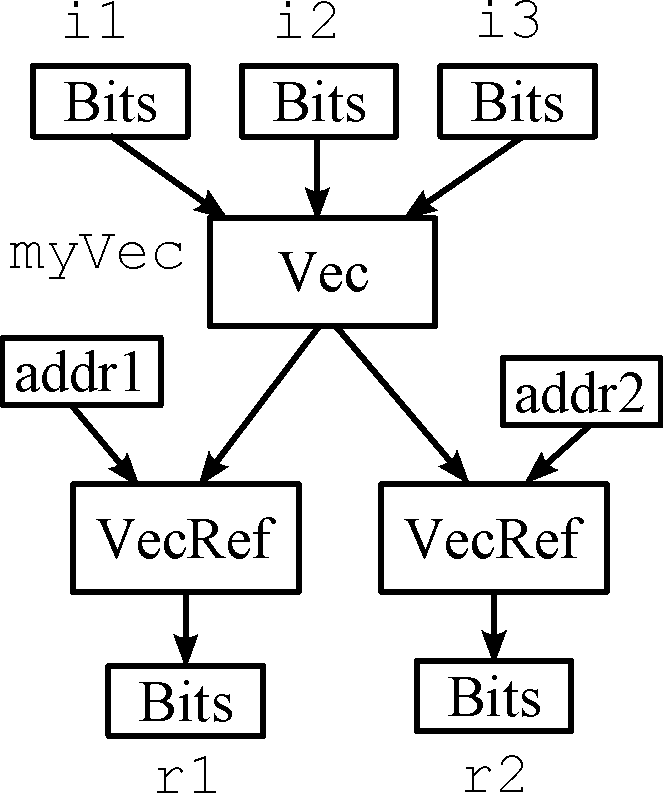
\includegraphics[width=0.5\textwidth]{figures/vecnode.pdf}
  \caption{{\bf Vec Node}. Example three entry {\tt Vec} with two
    read ports.}
  \label{fig:vecnode}
  \end{subfigure}
  \hfill
  \begin{subfigure}[t]{0.48\textwidth}
  \centering
  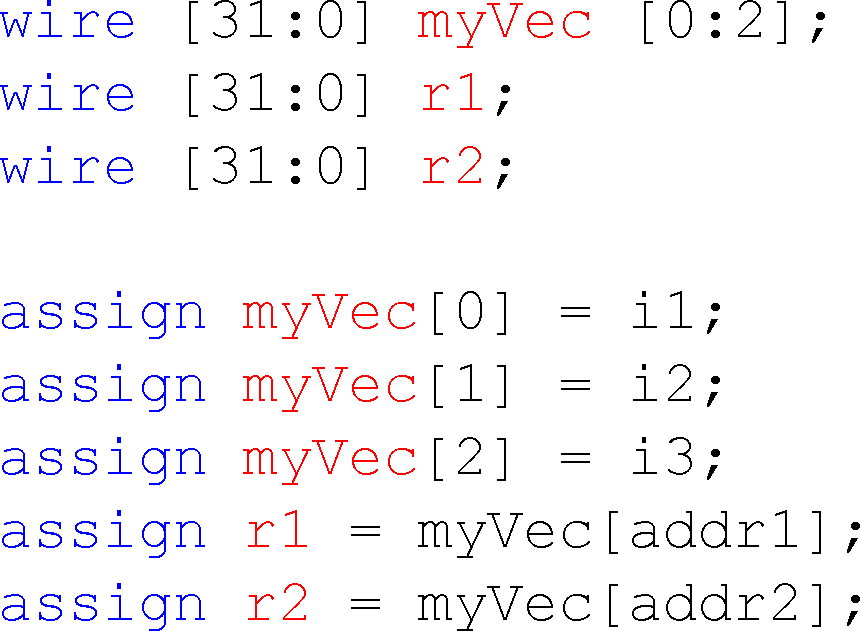
\includegraphics[width=0.7\textwidth]{figures/vecv.pdf}
  \caption{{\bf Generated Vec Code}. The two {\tt VecRef} nodes map to
  array accesses in Verilog.}
  \label{fig:vecv}
  \end{subfigure}
\caption{{\bf Vec}.}
\label{fig:vec}
\end{figure}

We use {\tt Vec} and {\tt VecRef} nodes to target 2-D Verilog arrays
from within Chisel. Vecs are useful for organizing small collection of
wires into an indexable structure.

\textbf{Vec Node}. The {\tt Vec} node maps directly to the 2-D Verilog
array. Users instantiate this node with the desired number of entries
and then populate the node using {\tt :=}
assignments. Figure~\ref{fig:vecnode} shows a 3-entry {\tt Vec} where
the user has connected {\tt i1-3} to the {\tt Vec}. The width of a
{\tt Vec} node is inferred to be the maximum width of its inputs (in
this example, 32-bits wide). {\tt Vec}'s {\tt emitDec} function will
return the string
\begin{align*}
\centering
\text{\tt{wire [width-1:0] vec\_name [0:entries-1];}}
\end{align*}
where {\tt vec\_name} is the name of the node, {\tt width} is the
inferred width, and {\tt entries} is the number of entries in the
{\tt Vec}. The {\tt emitDef} function emits an assign statement for
each entry in the Vec.

\textbf{VecRef Node}. After instantiating and populating the Vec,
users will want to access the {\tt Vec} with dynamic addresses. Each
access with a new address will make a new {\tt VecRef} node. The
inputs to a {\tt VecRef} node are an address and a 
{\tt Vec} and its inferred with is the width of its input
{\tt Vec}. Figure~\ref{fig:vecnode} two {\tt VecRef} nodes made from
accessing the same {\tt Vec} with two different addresses. 
{\tt VecRef}'s {\tt emitDec} simply declares the name and width of the
node. Its {\tt emitDef} entry will return the string
\begin{align*}
\centering
\text{\tt{assign ref\_name = vec\_name[addr];}}
\end{align*}
where {\tt ref\_name} is the name of the {\tt VecRef} node, 
{\tt vec\_name} is the name of the {\tt Vec} and {\tt addr} is the
address.
